%% ================================================================================
\chapter{Method}
\label{ch:method}
%% ================================================================================

\section{Data origin}
\label{sec:Data_origin}
%	-Data origin
%		-Fermi collaboration
%		-LAT
%		-Fermi FTOOLS
%		-point source subtraction
%		-pass7 vs pass8
%			-wider energy range
%			-better statistical and systematic errors
%			-better event selection




%(Maybe also some spectrum with pass7 and pass8 to see the differences.)

%\begin{figure}
% \centering
% 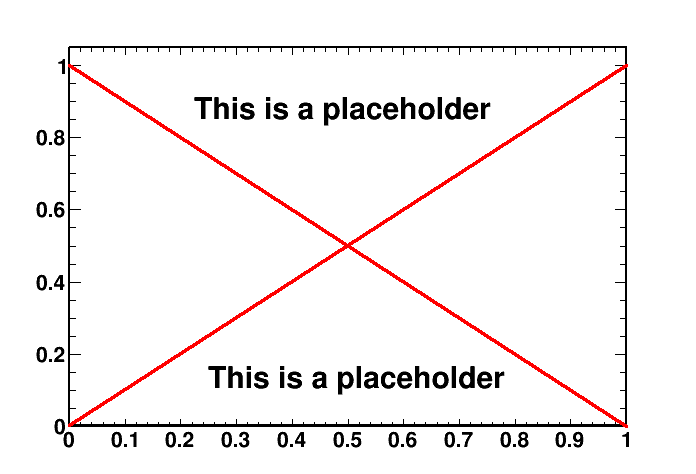
\includegraphics[width=.9\linewidth]{pic/dummy.png}
% \caption{Images of the exposure map}
% \label{fig:proton_spec}
%\end{figure}

\begin{figure}[h]
  \centering
  \begin{minipage}[h]{0.45\textwidth}
  	\centering
	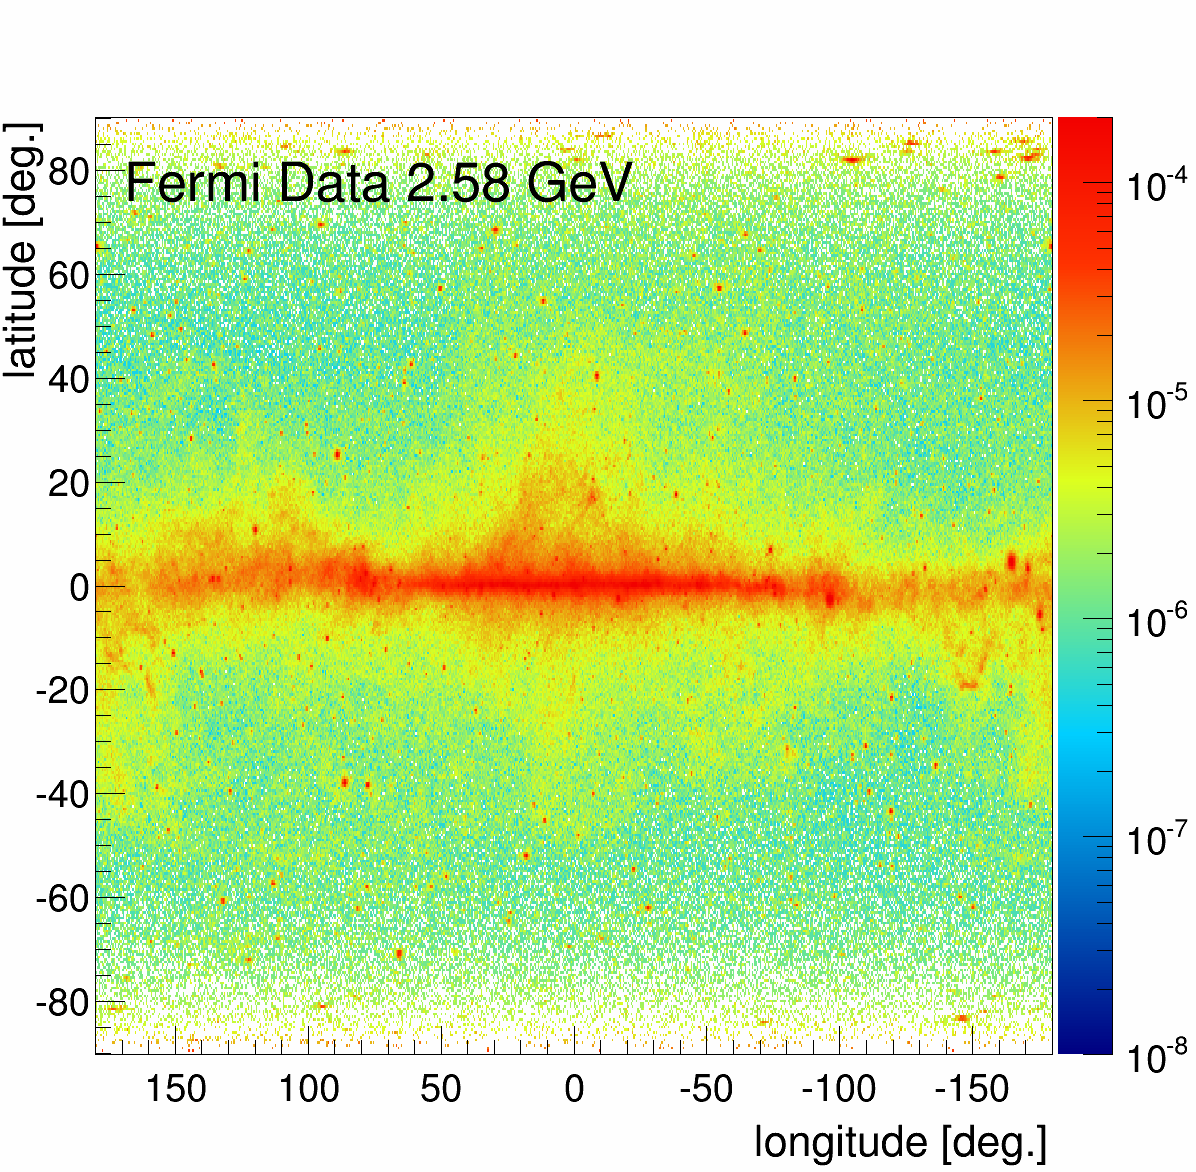
\includegraphics[width=1.\linewidth]{pic/method/Flux_FermiData_raw_E12.png}
  	\subcaption{}
  	\label{fig:raw_data}
  \end{minipage}
  \hfill
  \begin{minipage}[h]{0.45\textwidth}
	  \centering
	  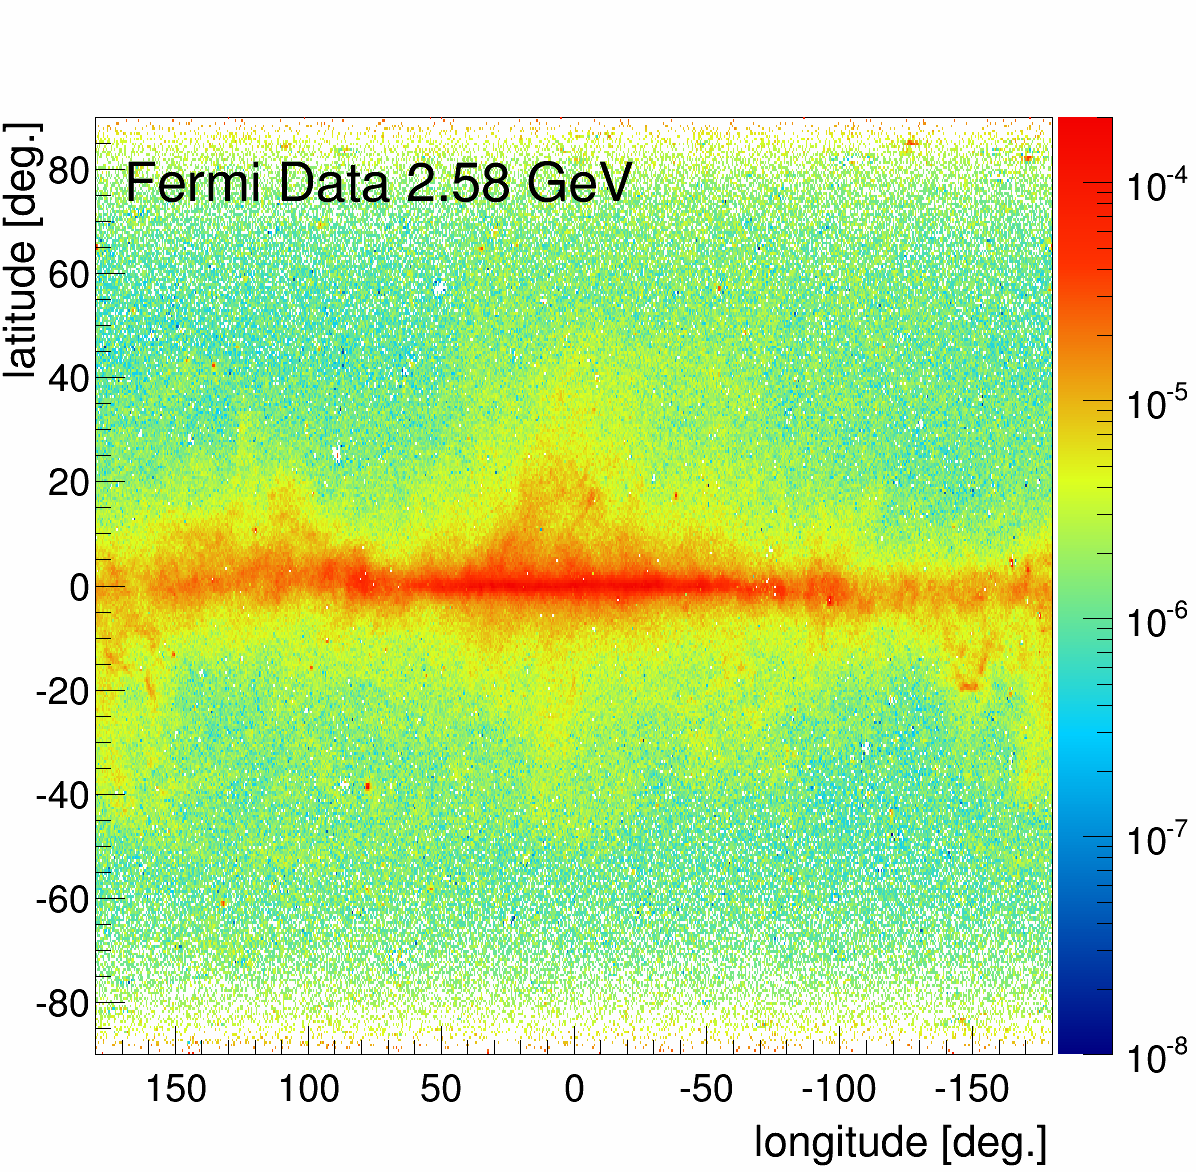
\includegraphics[width=1.\linewidth]{pic/method/Flux_FermiData-3FGL_E12.png}
	  \subcaption{}
	  \label{fig:data_ptsrc_subtracted}
  \end{minipage}
  \caption[Gamma-ray sky by Fermi.]{Map of the gamma ray sky as seen by the Fermi telescope around 2 GeV. Measured gamma ray flux before (left) and after (right) point source subtraction in $GeV/s/m^2/sr$. Most of the spots formed by point sources have disappeared, leaving only the diffuse background emission from CR. The subtraction does not remove all point sources, and can create artificial "holes" in the map (for example at coordinates (90, 25) or (50, 60)). These can be disregarded as relevant data, or can also disappear when using a larger binning.}
  \label{fig:method_pass8} 
\end{figure}

All the following work is based on the measurement of gamma rays coming from intra- and extra-galactic sources. The quality and accuracy of the data is one of the most important points that will determine the general quality of the results. Thus it is capital to be certain that the gathering and treatment were done properly.

The Fermi Large Area Telescope (LAT) observes the gamma-ray sky since 2008 and provides all the data of this work. \cite{Fermi2009}
All the information and data are available on the web and anybody can access them, using the tools given by Fermi. \cite{FermiTools}

The reconstruction method and data set of Fermi LAT is improved regularly, improving the statistics, the systematic errors and the point source subtraction. The latest data set to date, called Pass 8, is used for this work.
One of the most important steps in the treatment process is the selection of the events. Every photon measured is saved along with all its properties in a data file. Then this list is filtered to keep only the relevant observations. The filter can be based on the incoming direction, the energy or the time of observation, but also on the quality of the event reconstruction. This last cut can be critical. It will determine the chances that the measured event is in fact a gamma ray, and not some background noise polluting the data. The more strict the filter is, the less events are kept for analysis and the statistical errors increase. This work uses the CLEAN class recommended by the Fermi team for diffuse emission analysis. \cite{FermiTools}

The main parameters of the selection can be found in Tab \ref{tab:fermi_selection_parameters}.

\begin{center}
\begin{table}[h]
\centering
\begin{tabular}{|c|c|p{6.5cm}|}
\hline
\multicolumn{1}{|c|}{\textbf{Parameter name}} & \textbf{Parameter value} & \multicolumn{1}{c|}{\textbf{Description}}                                                                   \\ \hline
Event class                         & 256 (CLEAN)              & Quality parameter. Varies the level of background noise.                                                    \\ \hline
Event type                          & 3                        & Back+front event.                                                                                           \\ \hline
Time boundaries                     & INDEF                    & Selecting all events since beginning of observation.                                                        \\ \hline
Minimum energy (MeV)                & 58.4731                  & Minimum energy of the event.                                                                                \\ \hline
Maximum energy (MeV)                & 513056                   & Maximum energy of the event.                                                                                \\ \hline
zmax (degrees)                      & 90                       & Maximum zenith angle to get rid of the Earth contaminations, as recommended by the LAT instrument team. \\ \hline
\end{tabular}
\caption[Main parameter for Fermi data selection.]{List of the main parameters used for data selection. The exact script can be found in the appendix.}
\label{tab:fermi_selection_parameters}
\end{table}
\end{center}
\todo{add code in appendix and ref}


Another important point is the creation of the exposure map. It tells how long the telescope spent observing a given part of the sky. After dividing the count map by the exposure, a flux map is obtained that does not depends on the observation time of particular regions. For example, if the telescope observed the galactic center ten times more often than the Orion nebula , there is no way to know at first if the higher counts in the GC is due to the longer exposition time or a higher flux from this region.
%It is used to correct an observation bias. 

The goal of this work is to study the diffuse sources of gamma-rays from inside and outside the Milky Way. Of course, the LAT does not differentiate them from point source gamma-rays. This has to be done manually as the last step in the treatment process. A catalog of gamma ray point sources (3FGL) is available on-line on NASA website \cite{3FGL2015}. This catalog lists most of the known and identified point sources, along with their spectral shape and flux. This information can then be used to model the number of counts coming from point sources and their spatial and energetic distribution. To achieve this, the point sources properties must be combined with the instrument properties. The point source flux is multiplied by the LAT exposure time corresponding to its position. This flux must also pass through the instrument and its defaults will deform the initial shape of the source. For a point source, the final image obtained by the detector is the Point Spread Function (PSF) of the telescope and is given with the Fermi tools. Every point source is convoluted by the PSF corresponding to the initial event selection, creating the final point source map as would be observed by the instrument.
Once this model map is obtained, it is subtracted from the data to only keep the diffuse emission (see Fig. \ref{fig:method_pass8}). Since the models are never perfect and all point sources are not listed, errors or anomalies in the observations can appear. Keeping the dataset up-to-date allows to use the latest catalogs and best reconstruction.


Once all the data treatment is done, a flux map of the entire sky in $counts/s/m^2/GeV/sr$ is produced. The map is divided in bins of $0.5 \times 0.5$ degrees on a Cartesian projection, also called cones. Every bin contains 30 logarithmic energy bins ranging from 60 MeV to 513 GeV with a 1.2 multiplicative step. Thus the final data cube is of dimension $720 \times 360 \times 30$. For visibility purposes, every energy bin is multiplied by its energy squared, becoming an energy flux in $GeV/s/m^2/sr$. This will be the default units used for the rest of this work.

The errors on the data are coming from two sources. First are systematic errors introduced by the instrument or the treatment process. They are around 3\%, but can increase for low or high energies (Fig. \ref{fig:LAT_sys_err}). These errors have multiple causes, mainly the PSF and the energy resolution (or energy dispersion) of the instrument. The plot shows how the systematic errors vary when correcting, or not, for these effects. The treatment shown in appendix accounts for energy dispersion.
The second source is the statistical errors, proportional to the square root of counts. This property will make them decrease when the acquisition time will increase. They are dominant at high energy (above 50 GeV) where fewer events are observed. On contrary at low energies (around 100 MeV), the systematic errors dominate. The final equation is the following :

\begin{equation}
\sigma_{tot} =\sqrt{\sigma_{sys}^2 + \sigma_{stat}^2} = \sqrt{\sigma_{sys}^2 + \frac{1}{N}}
\end{equation}


\begin{figure}[h]
 \centering
 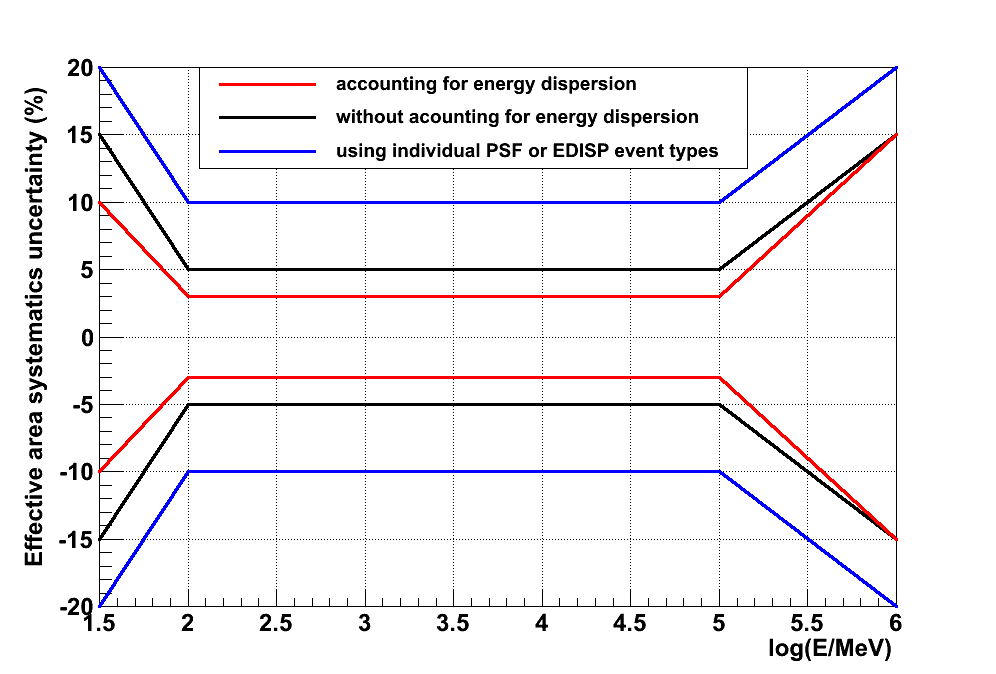
\includegraphics[width=.6\linewidth]{pic/method/LAT_sys_error.png}
 \caption[Systematic errors for the Fermi LAT]{Systematic error for Pass 8 data as a function of the energy and the treatment procedure. The energy dispersion is the energy resolution of the instrument; this effect is known and can be corrected (in red), lowering the systematic errors. This is what was done for this study. The black line does not account for energy dispersion. The blue line shows the systematics for specific event types, and is used only for specific that can be ignored. The few percent gained with the energy dispersion treatment at very low energies (below a few hundred MeV), where the statistical uncertainties are not dominant any more, can be critical.}
 \label{fig:LAT_sys_err}
\end{figure}




\newpage
\section{Model components}
\subsection{From CRs to gamma-rays}
%Add subsection on how the gamma spectra are calculated. Don't forgt to explain how the 3 IC comps are managed}

The gamma-ray spectra used in this study are directly calculated from the CR spectra. The next section describes the CR distribution used to get the gamma-ray spectra corresponding to the modeled processes. Once the CR spectrum is defined, a propagation software \cite{Evoli2008}, DRAGON, is used to determine the emitted gamma-ray spectrum. For most of the components, the spectral shape does not vary depending on the direction, only its normalization does.%, but that does not play a role in the fitting method (cf \ref{sec:fitting_method}).
DRAGON uses a model of the galaxy (ISRF, matter distribution, etc...) and the input CR spectra for protons and electrons to produce gamma-ray spectra as an output for pion decay, bremsstrahlung and inverse compton scattering.


\subsection{Basic components}
%	-3 Basic components
%		-PCR
%			-proton CR follow power-law E^-2.849
%			?-try with break at 5-10GeV with index ~ -2.7 ?
%		-IC and BR
%			-electron CR spectrum E^-3.21
%			-break at 1GeV, index E^-3.21 + 2.4 below break

\begin{figure}[h]
  \centering
  \begin{minipage}[h]{0.45\textwidth}
  	\centering
	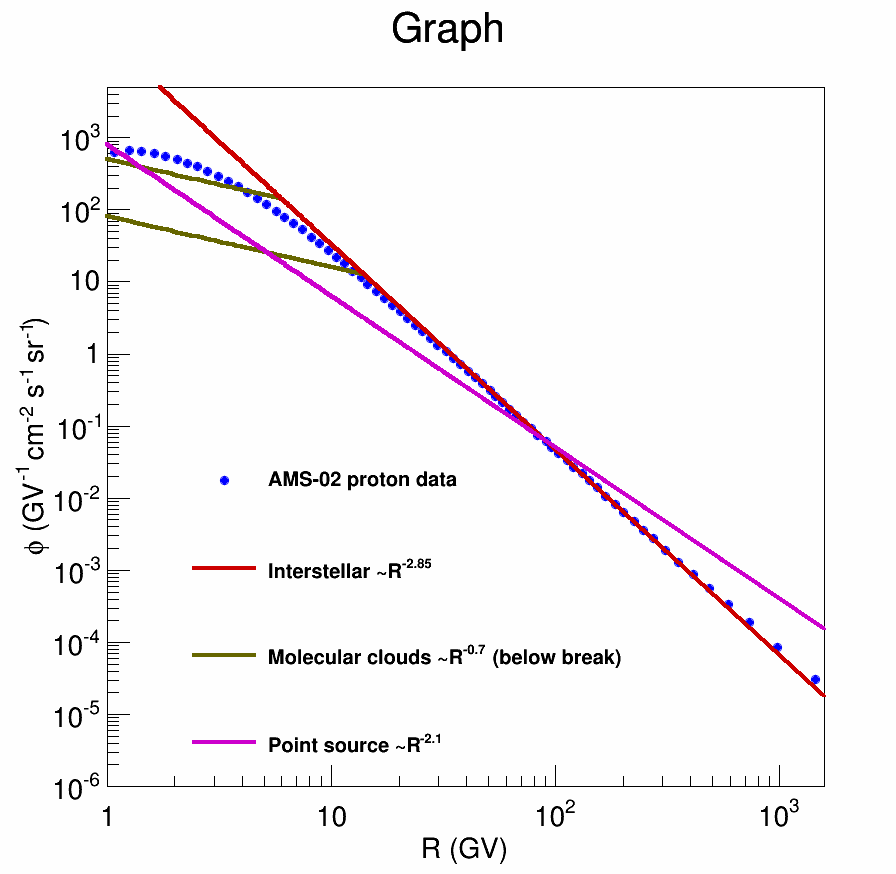
\includegraphics[width=1.\linewidth]{pic/method/./CR_protons_spectra.png}
  	\subcaption{}
 	\label{fig:proton_spec}
  \end{minipage}
  \hfill
  \begin{minipage}[h]{0.45\textwidth}
	  \centering
	  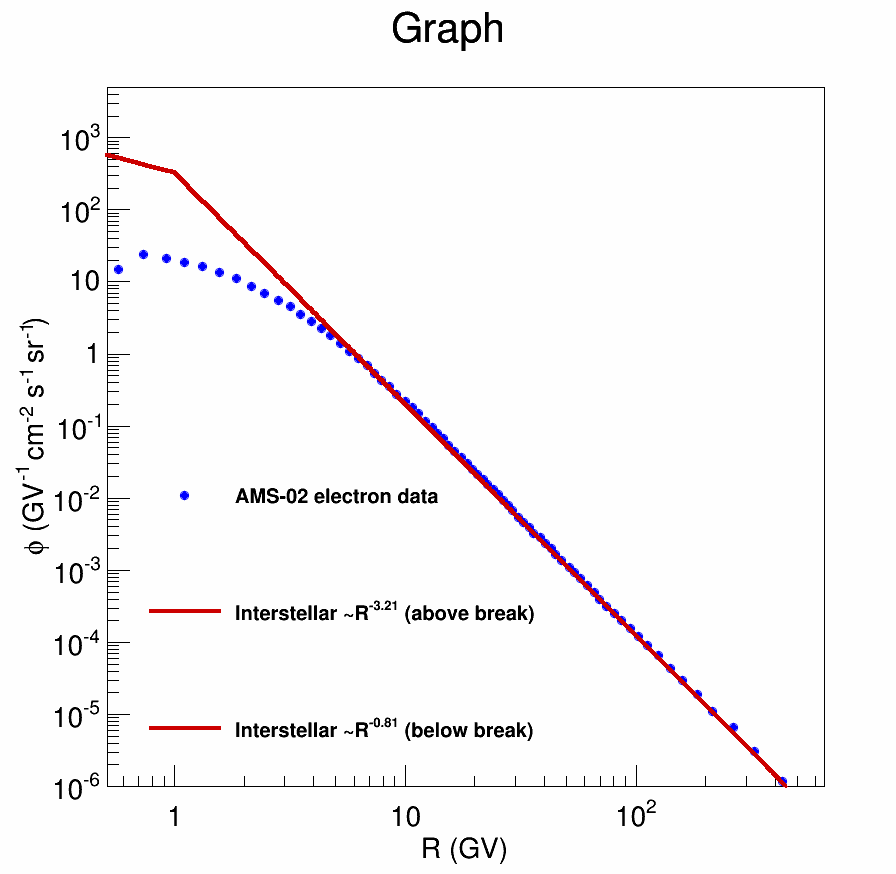
\includegraphics[width=1.\linewidth]{pic/method/./CR_electrons_spectra.png}
	  \subcaption{}
	  \label{fig:electron_spec}
  \end{minipage}
  \caption[Initial CR spectra.]{Cosmic Ray spectra used to determine the gamma-ray templates. (a) Power-law proton spectra used to produce the proton based templates. In comparison, the measured data by AMS-02. The MC spectrum breaks are varying between the two shown here. Above the break, the index is the same than or propagated CR. (b) Power-law electron spectrum used to produce the IC and BR templates, compared once again with AMS-02 data. This time a break is introduced at 0.2 GeV.}
  \label{fig:cosmic_ray_spec}
\end{figure}


\subsubsection{$\pi^0$ production by propagated cosmic rays (PCR)}

%%% ARTICLE
The initial propagated proton spectrum for the PCR template is obtained from the observed proton data from AMS-02 \cite{Aguilar15}. A good approximation is an unbroken power law ($R-\alpha$) with a spectral index ($\alpha$) of 2.85 at rigidities above 45 GV. At lower rigidities, the flux is not described by the power law because of solar modulations \cite{Gleeson68}, as seen in Fig. \ref{fig:proton_spec}. %To find the best parametrization, several indexes and breaks were tested. The optimal parametrization was found by interpolation between the fits with the best test statistic. Finally, the gamma-ray data are well described by an unbroken power law for the protons with a spectral index ($\alpha$) of 2.85 at all rigidities.\\
%%% ARTICLE

%There is also the possibility to introduce a break around a few GeV, to have a slightly harder spectrum at lower energies.\\


\subsubsection{Inverse Compton (IC) and bremsstrahlung (BR)}

\begin{figure}[h]
  \centering
  \begin{minipage}[h]{0.45\textwidth}
  	\centering
	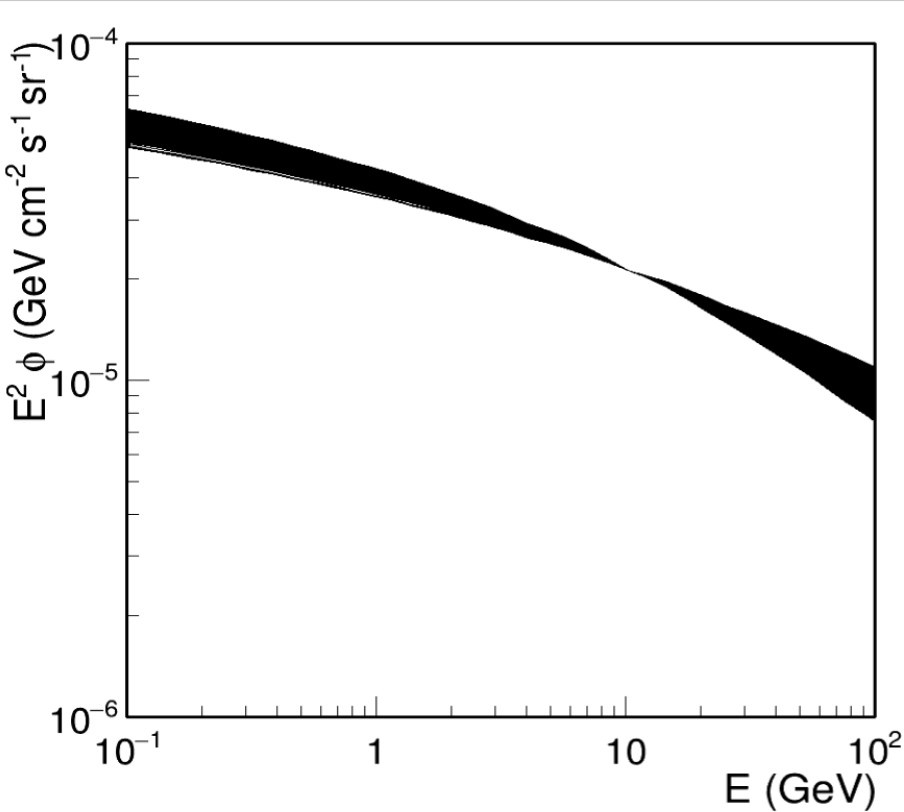
\includegraphics[trim={0 0cm 0 0.2cm}, clip, width=1.\linewidth]{pic/method/IC_variations.png}
 	\subcaption{}
 	\label{fig:IC_variations}
  \end{minipage}
  \hfill
  \begin{minipage}[h]{0.45\textwidth}
	  \centering
	  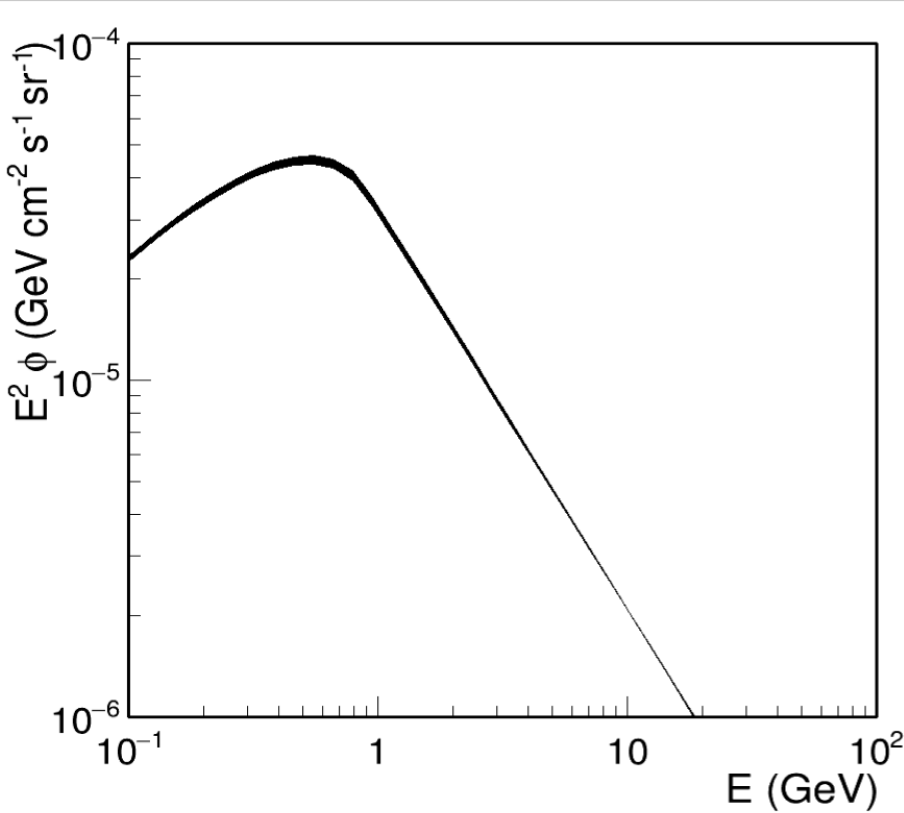
\includegraphics[trim={0 0cm 0 0.2cm}, clip, width=1.\linewidth]{pic/method/BR_variations.png}
	  \subcaption{}
	  \label{fig:BR_variations}
  \end{minipage}
  \caption[Variations of the IC and BR template over the sky.]{(a): Superposition of the inverse compton scattering template in every sky direction, normalized arbitrarily at 10 GeV. (b): Superposition of the bremsstrahlung template in every sky direction, normalized at 10 GeV. The CR electron spectrum use here has a break at 1 GeV, but its position does not influence the spatial variations. The variations of BR are very small and can be neglected.}
  \label{fig:IC_BR_variations} 
\end{figure}


The interstellar electron spectra need a break around 0.2 GeV with a spectral index of 3.21 above. This is compatible with the locally observed electron spectrum (see Fig. \ref{fig:electron_spec}). Below the break the optimal spectral index is 0.81, which implies a suppression of electrons. %The break point might be related to the fact that around 0.2 GeV electrons have the smallest energy losses, since above this energy synchrotron, BR and IC dominate the energy losses, while below this energy ionization losses become strong, thus depleting the electron spectrum below 1 GeV. A similar break in the electron spectrum was needed in the Fermi diffuse model \todo{cite[46]}.\\
The targets for the production of gamma-rays are the interstellar gas for BR and the interstellar radiation field (IRF) for IC, which are both strongly dependent of position%The latter consists of photons from the cosmic microwave background, the infrared radiation from hot matter, like dust and the star light
, so the photon composition varies with sky direction.
For this reason, the IC and BR templates are calculated for each sky direction. The variation over the sky is about $\pm 10\%$, as shown in \ref{fig:IC_variations}. 
The BR template only depends on the interstellar gas distribution, decreasing the variations considerably compared to IC, as shown in \ref{fig:BR_variations}.
%Note that the intensity of photons in the interstellar radiation field nor the gas density play any role in a template analysis, since the intensity of each contribution to the gamma-ray sky is determined by the fitted normalization factors in Eq. 1.



%The IC and BR spectra are both obtained from the interstallar electron distribution, taken here as a broken powerlaw with a break \todo{at 1GeV}. The index is 3.21 over the break and 0.8 below.
%The IRF is composed in the mostly by starlight (UV), and in with smaller contribution dust emission (IR) and the cosmic microwave background. The first two components of the IRF are position dependant, and this is why we have to calculate the IC spectrum for every sky direction.
%The BR component is directly linked to the gas, and charged particles distribution. This is also a reason too calculate the BR component in every sky directions. The variations are not too large.




\subsection{Additional components}
%	-2 or more additional components:
%		-SCR
%			-proton CR follow power-law E^-2.1
%		-MCR
%			-proton CR follow power-law E^-2.849
%			-break between 6 and 14GeV, index E^-2.849 + 2.149 below break
%		-DM
%			-Dark Susy
%			-Determination of Mass using best fit in CMZ
%		-MBR
%			-electron CR spectrum E^-3.21
%			-break between 6 and 14 GeV, index E^-3.21 + 2.4 below break
%	-Isosky
%		-Calculated from fermi model and adjusted in our fit

\begin{figure}[h]
  \centering
  \begin{minipage}[h]{0.45\textwidth}
  	\centering
	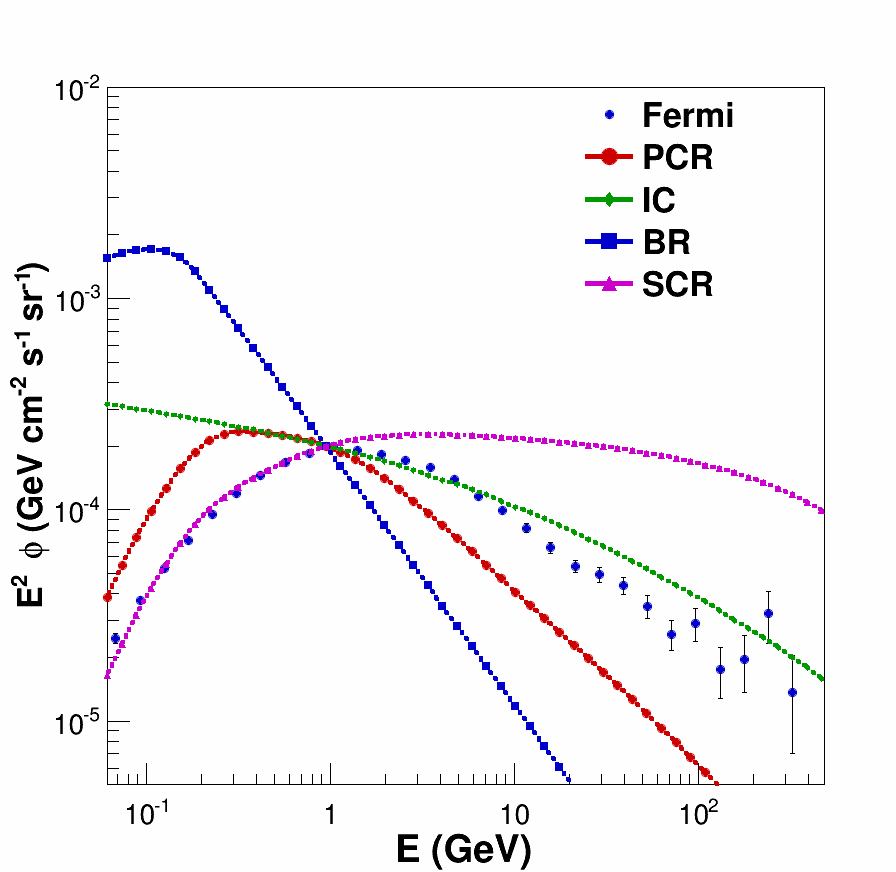
\includegraphics[width=1\linewidth]{pic/method/norm_bkg_comp.png}
  	\subcaption{}
 	\label{fig:norm_bkg_component}
  \end{minipage}
  \hfill
  \begin{minipage}[h]{0.45\textwidth}
	  \centering
	  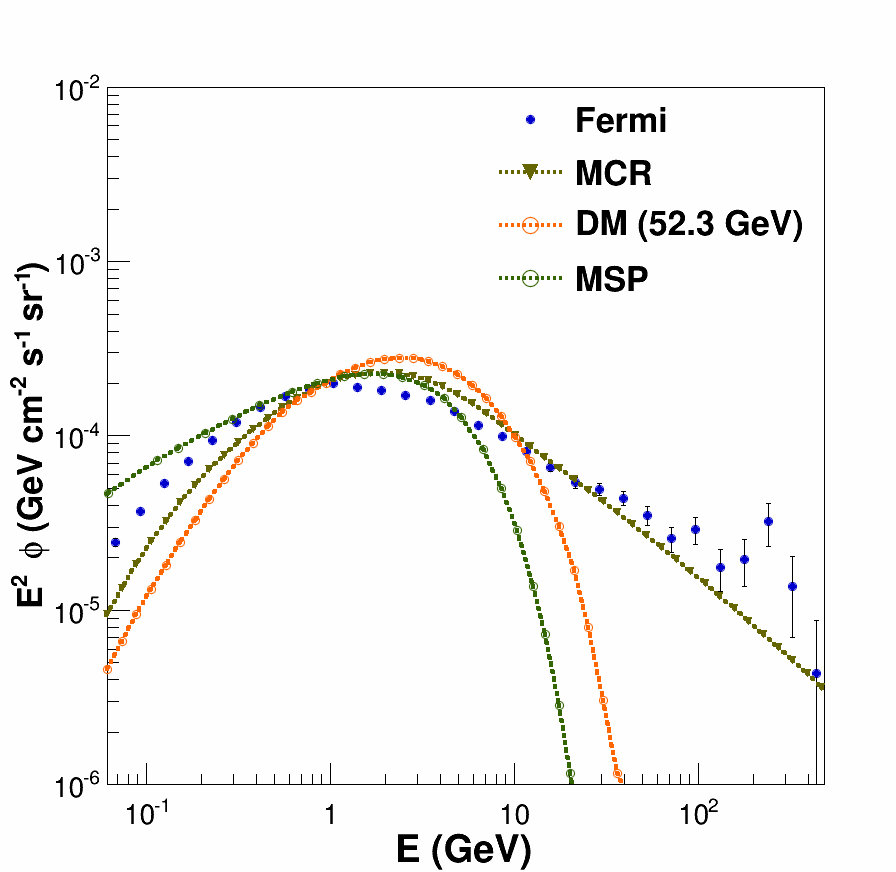
\includegraphics[width=1\linewidth]{pic/method/norm_excess_comp.png}
 	  \subcaption{}
 	  \label{fig:norm_excess_component}
  \end{minipage}
  \caption[Comparison of gamma-ray templates]{(a) Comparison of PCR, IC, BR and SCR templates, normalized at 1 GeV. Measured data from the central molecular zone is shown as well. All four components have very different spectrum and index that make them easily identifiable by the fit. (b) Comparison of the three excess components, along with the data from the CMZ.}
  \label{fig:norm_spectra} 
\end{figure}




%
%\begin{figure}
% \centering
% 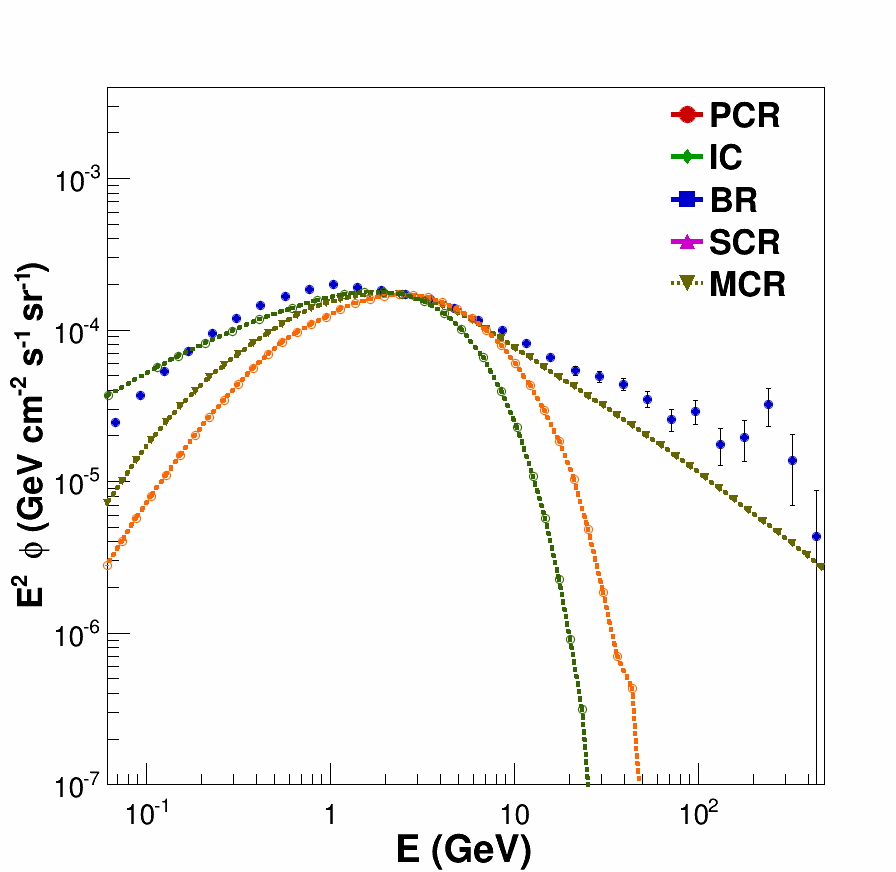
\includegraphics[width=.5\linewidth]{pic/method/excess_comp.png}
% \caption{The three excess component, compared with the data from the central molecular zone.}
% \label{fig:excess_component_comp}
%\end{figure}

\subsubsection{$\pi^0$ production by source cosmic rays (SCR)}

%%% ARTICLE
The proton spectra producing the SCR template can be described by a power law with a spectral index of 2.1, as obtained from the best gamma-ray template fit. The index 2.1 for the SCR template %agrees with the data from the Fermi Bubbles, shown by the data points inside the shaded band in Fig. \ref{fig:proton_spec}; the index 2.1 
is expected from diffuse shock wave acceleration. \cite{Biermann10} \cite{Hillas2005} 
The source CRs are accelerated, or escape from the galaxy, hence a harder spectrum at high energies compared with propagated CR spectrum is expected.

%The fact that the Fermi Bubbles and the cosmic rays inside sources have the same spectrum strongly suggests that they are connected by point sources providing advective outflows of gas in the Galactic center. \todo{cite[44]}
%%% ARTICLE

\subsubsection{$\pi^0$ production by molecular clouds cosmic rays (MCR)}

%%% ARTICLE
A proton spectrum with broken power-law can be used to parameterize the decreasing gamma-ray emissivity from MCs below 2 GeV. The break can vary from 6 to 14 GeV for different clouds according to the fit. Above the break an optimal spectral index of 2.85 was found to be the same as for the PCR spectrum, as expected if the high energy propagated protons are above a certain magnetic cutoff. Below the break, the spectral index is 0.7, thus providing a significant suppression of protons below the break, as can be seen from Fig. \ref{fig:proton_spec}. This lower break spectral index does not have a strong influence on the fit and therefore is taken to be 0.7.
%Energy losses alone cannot reproduce such a suppression of the proton spectrum below the break, but magnetic cutoffs are able to do so. Such a cutoff is well known from cosmic rays entering the Earth's magnetic field: particles below typically 20 GV entering near the magnetic equator do not reach the Earth, but are repelled into outer space by the geomagnetic cutoff. \todo{cite[62]} The rigidity cutoff of 20 GV is proportional to the magnetic moment. Although the magnetic field near the Earth (0.5 G) is orders of magnitude higher than the typical magnetic fields in dense MCs \todo{cite[63]}, the much larger sizes of MCs - or its substructure of filaments and cloudlets \todo{cite[64]} - yield magnetic moments of the same order of magnitude as the Earth's magnetic moment, so similar magnetic cutoffs are plausible. 
Variations in the magnetic cutoff in MCs are expected from the variations in size and in magnetic field, the latter increasing with MC density. \cite{Crutcher2012} 
These variations, between 6 and 14 GeV, make the position of the gamma-ray spectrum maximum vary around a few GeV.
%The fit prefers a constant spectral index below the break for all sky directions. Such a constant spectral index is plausible with regular magnetic fields oriented in the disk %\todo{cite[65, 66]} 
%and the "cloudlets" inside MCs %\todo{cite[64]} 
%form magnetic dipole fields. Then the largest cutoff occurs for cosmic rays entering from the halo perpendicular into the cloud for any orientation of the magnetic dipole. For a given entrance angle the cutoff would provide a sharp break, but for an isotropic distribution of entrance angles the break points are smeared. A distribution of break points will provide a slope below the maximum break determined largely by the isotropic distribution of the entrance angles into the disk. Since this distribution is the same for all MCs the slopes below the break will be similar for all MCs, even if the maximum break varies.
%%% ARTICLE

%
%The MCR component is produced by the same process than for PCR, but with a different proton distribution. Due to the magnetic cut-off in MCs, we introduce a break in the proton spectrum between 6 and 14GeV. We leave the index above to 2.85 as for PCR as expected, but we reduce it to 0.7.\\
%
%The magnetic fields around such clouds are not as strong than what we have in the solar system, but the spatial scales are much bigger and could produce such a break. Of course it position may vary from clouds to clouds and it is why we choose to free its position when fitting.\\
%
%This gives us a spectrum peaking around 2GeV.




\subsubsection{Dark matter annihilation (DM)}

%%% ARTICLE
Dark matter particles are expected to annihilate and produce hadrons of roughly twice the WIMP mass, just like in electron-positron annihilation. This would be a large contribution to gamma-rays via $\pi^0$ decays. A smaller fraction of WIMP annihilation can lead to $\tau$ lepton pairs, which can lead to $\pi^0$ production in the hadronic $\tau$ decays. This contribution is expected to be small and is neglected. The DM template can be calculated with the DarkSusy software. \cite{Gondolo2004} \cite{Gondolo2005}
An annihilation signal peaking around 2-3 GeV requires a WIMP mass around 50 GeV, as shown in Fig. \ref{fig:norm_excess_component}. 
The DM template falls down to zero for energies above twice the WIMP mass, which make it a softer spectrum than MCR. 
%%% ARTICLE

%
%The DM spectrum is calculated using the DarkSUSY software. Since the initial WIMP mass is not known, we chose to let the fit decide in the CMZ region and fix it to this value in the other regions. The value generally turns around 50GeV, which make the gamma-ray spectrum peak around 2GeV.


\subsubsection{Milli-second pulsars gamma-ray production (MSP)}

The MSP template is directly taken from the Fermi study \cite{Fermi2017}. It simulates the emission of 1700 milli-second pulsars with different energies around the galactic center.
The high energy shape of the spectrum closely resemble the DM template, but the main difference with DM and MCR is for low energies. Indeed, below 1 GeV, the MSP template is a lot softer and this feature makes it discernible from MCR and DM.

\subsubsection{Isotropic component}

\begin{figure}
 \centering
 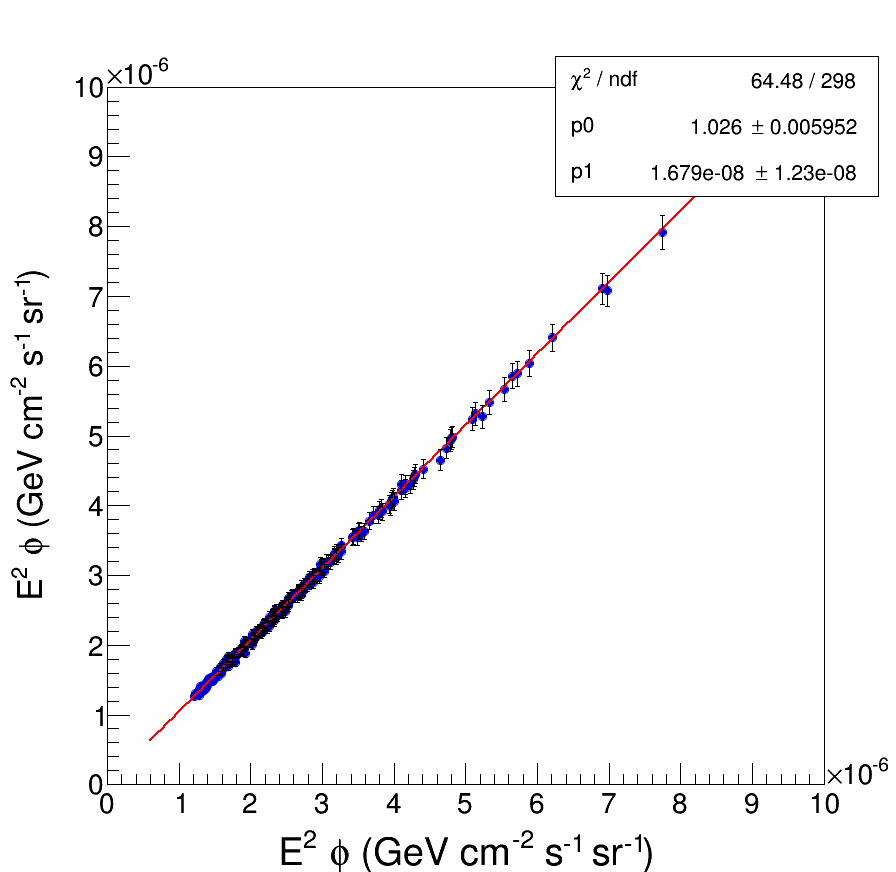
\includegraphics[width=.5\linewidth]{pic/method/iso_calibration.png}
 \caption[Isotropic calibration.]{The fitted flux versus the observed flux data in every region of the sky for a given energy of 1 GeV. A linear fit is performed to find the offset p1 at the vertical axis. This number represents the amount the isotropic component shifts the data in all cones. Once this is done for every energy bin, the offset is added to the previous isotropic template and the process is repeated until convergence. }
 \label{fig:iso_calibration}
\end{figure}


%%% ARTICLE
The isotropic template represents the contribution from the isotropic extragalactic background and hadron mis-identification. Its spectral shape and absolute normalization are provided within the Fermi software \cite{FermiTools}, but it was redetermined for the analysis as follows.
A first fit of the data in regions outside the bubbles and the galactic disk using the isotropic template from the Fermi software is produced as an initial estimate. This fit takes into account all components of the best fit available.
If one plots the total observed gamma-ray flux versus the fitted flux in the various cones in a certain energy bin, one expects a linear relation crossing the origin if the isotropic flux is estimated correctly (See Fig. \ref{fig:iso_calibration}). However, if the isotropic contribution is either too low or too high, an offset at the origin is introduced in the linear relation. Since the isotropic component is by definition the same for all cones for a given energy, this offset can be subtracted from the Fermi template to improve the fit. 
%An example of such a fit is shown in Figure \ref{fig:iso_calibration} for an energy bin between \todo{3.7-5.2 GeV}. 
Once the offset is determined for each energy bin and subtracted from the original template, the process is repeated until the offset converges to zero. This process is illustrated in its four first steps in the appendix \ref{app:app_iso_process}.

%The linear relation between data and fit is always supposed to have a slope of one, or the process does not converge.
%The resulting template in our analysis has deviations from the Fermi template up to $35\%$ above 2 GeV, as shown in the insert of \ref{fig:iso_calibration}.
%%% ARTICLE

\newpage
\section{Fitting method}
\label{sec:fitting_method}
%My method:
%	-Spectral templates fitted to the data
%		-independant spatial cones on the entire sky (usually 797 for optimized sizes)
%		-minimum chi2 fit using ROOT for every cone
%		-Benefits
%			-energy related features
%			-only a few degrees of freedom -> Well constrained fit (5(or 6) dof against 21-30 points)
%		-Downside:
%			-No spatial templates. (only the isosky)


The fitted data can be seen as a data cube whose dimension are longitude, latitude and energy. The finest spatial grid is divided in $720 \times 360$ cones of $ 0.5^\circ \times 0.5^\circ $. Every cone contains 30 energy bins. This allows to treat different portions of the sky independently of one another.
(((Since the cones do not have the same solid angle and the statistics in a small binning is low, the grid is more often composed of 797 bins of different sizes, bigger at the poles and smaller near the equator. This allows for higher statistics in lower flux regions and where a high spatial resolution is not needed (i.e. at high latitudes). In the same time, the equator and the GC have a lot more counts and can be treated in a smaller binning. This binning is faster to compute than a regular grid with an good enough output quality to study the results.)))

The fit uses a certain number of components (three at least) each corresponding to a certain phenomenon and described earlier. They all have certain energy spectra that can vary with the position in the sky in the case of IC (See Fig. \ref{fig:norm_spectra}).

The fits are done for every bin independently. After choosing the templates used for the fit, their scaling factor is the only degree of freedom allowed. Using a ROOT TVirtualFitter object, every template is scaled up or down until its sum comes the closest to the data. So the modeled flux is given by:

\begin{equation}
\phi(E,l,b) = \sum_{i=1}^{n} a_i(l,b)*T_i(E,l,b)
\end{equation}

where $\phi(E,l,b)$ is the total fitted flux at energy $E$, longitude l and latitude b, n is the number of components used in the fit, $a_i(l,b)$ is the scaling factor of component $i$ at position $(l,b)$ and $T_i(E,l,b)$ is the $i^{th}$ component's model flux. Only the IC and BR component depends on the longitude and latitude, and the isotropic template has a fixed scaling factor.

Mathematically, the minimum distance between the model and the data is found when the $\chi^2$ value is lowest. It is calculated as follows:

\begin{equation}
\chi^2 = \sum_{i=1}^{30} \left[ \frac{ \left( D_i - \sum_{j=1}^{n} \left[ (a_jT_{ij})^2 \right] + iso \right) ^2}{\sigma_i^2} \right]
\end{equation}

where:
\begin{itemize}
\item $D_i$ is the data flux in the $i^{th}$ energy bin.
\item $a_j$ is the scaling factor for the $j^{th}$ model component.
\item $T_{ij}$ is the model flux of the $j^{th}$ in the $i^{th}$ energy bin.
\item $\sigma_i$ is the geometric mean of the statistical and systematical error of the Fermi data point $i$.
\end{itemize}

The MCR break position does not vary in a single fit. A fit is done for different values of the MCR break independently, and the one with the smallest $\chi^2$ is kept. This break position is not counted as a degree of freedom in the fit.

The fit is very well constrained with only five or six degrees of freedoms depending on the model against 30 data points. A useful value is the $\chi^2 / d.o.f$ where $d.o.f = \#data\ points - \#free\ parameters - 1$. Thus, if a model describes data completely within its uncertainty, $\chi^2 / d.o.f = 1$, making the comparison between different fits easier. This rescaling will be applied every time when speaking about $\chi^2$ in the rest of the discussion, except if explicitly told. 
The closest a $\chi^2$ value is to one, the better the model follows the data. The higher it gets, the lower the quality of the fit. It can also happen that it gets lower than one. This can happen when the error bars on the data are too big.


Since every bin is fitted independently, it is not possible to implement a spatial template, i.e. where the spatial shape of a component would be fixed in advance. For example a component with a spherical distribution around the GC, as has been done in other works \cite{Calore2015}, \cite{Daylan2016}. It is used to let the fit find reasonable shapes by itself, only using the $\chi^2$ minimization technique.

%\section{Introduction of results}

This fitting method offers many ways to look at the results, depending on the interest. It is possible to produce flux maps of each component to study their spatial shapes at different energies. This can for example show a correlation between a certain template and a galactic feature such as the disk or the bubbles. Another way is to create a spectrum of one cone to look at the relative quantity of every template at different energies. This can put into evidence issues within the models and help improve the spectral shape of the components.

The first step when testing a new model is to see if it can reproduce results of previous studies. Only once it works and can be confidently used, can it produce new results.

%The next chapter will describe these results, first reproducing old studies, and 

%Recreation of previous studies (GC excess, problems).\\
%Introduction of new component to take care of those problems (SCR for high energies, MCR, Dm or MSP for 2GeV excess)


%%	-Weniger plots
%%		-study of spectra slope between 0.3 and 2 GeV
%%	-Specklings
%%		-Study of symmetry
%%	-Comparison with CO map
